\subsubsection{String patching (Win32)}

Possiamo facilmente trovare la stringa ``hello, world'' all'interno del file eseguibile utilizzando Hiew:

\begin{figure}[H]
\centering
\myincludegraphics{patterns/01_helloworld/hola_edit1.png}
\caption{Hiew}
\label{}
\end{figure}

E possiamo cercare di tradurre il messaggio in spagnolo:

\begin{figure}[H]
\centering
\myincludegraphics{patterns/01_helloworld/hola_edit2.png}
\caption{Hiew}
\label{}
\end{figure}

Il testo in spagnolo è più corto di un byte rispetto a quello inglese, quindi abbiamo aggiunto anche il byte 0x0A al fondo (\TT{\textbackslash{}n}) con un byte zero.

Funziona.

E se volessimo inserire un messaggio più lungo?
Ci sono alcuni byte a zero dopo il testo in inglese.
E' difficile stabilire se possono essere sovrascritti: potrebbero essere utilizzati da qualche parte all'interno del codice \ac{CRT}, oppure no.
Ad ogni modo, sovrascrivili solo se sai esattamente cosa stai facendo.

\subsubsection{String patching (Linux x64)}

\myindex{\radare}
Proviamo a modificare un eseguibile Linux x64 utilizzando \radare{}:

\lstinputlisting[caption=\radare{} session]{patterns/01_helloworld/radare.lst}

Questo è il procedimento: ho cercato la stringa \q{hello} utilizzando il comando \TT{/},
poi ho impostato il \emph{cursore} (\emph{seek}, in \radare{}) a quell'indirizzo.
Poi voglio essere sicuro di essere veramente nel posto giusto: \TT{px} mostra un dump dei dati locali.
\TT{oo+} imposta \radare{} in modalità \emph{read-write}.
\TT{w} scrive una stringa ASCII nel \emph{seek} corrente.
Nota il \TT{\textbackslash{}00} al fondo---è un byte zero.
\TT{q} esce (quit).

% TBT
%\subsubsection{This is a real story of software cracking}
%\label{\SoftwareCracking}
%
%An image processing software, when not registered, added watermarks,
%like ``This image was processed by evaluation version of [software name]'', across a picture.
%We tried at random: we found that string in the executable file and put spaces instead of it.
%Watermarks disappeared.
%Technically speaking, they continued to appear.
%\myindex{Qt}
%With the help of Qt functions, the watermark was still added to the resulting image.
%But adding spaces didn't alter the image itself...

\subsubsection{La \emph{traduzione} del software all'epoca del MS-DOS}

Questo era un metodo comune per tradurre i software per MS-DOS durante gli anni '80 e '90.
A volte le parole e le frasi sono leggermente più lunghe rispetto ai corrispettivi in inglese, per questo motivo i software \emph{adattati}
hanno molti acronimi strani ed abbreviazioni difficili da comprendere.

\begin{figure}[H]
\centering
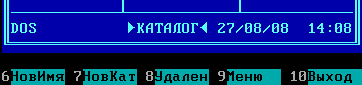
\includegraphics[width=0.5\textwidth]{patterns/01_helloworld/Norton_Commander_v5_51.png}
\caption{\ITph{}}
\end{figure}

Probabilmente questo è successo in molti Paesi durante quel periodo.
